% =====================================================================
%  c01：原印刷页 5–13（PDF p.6–14）
%  §1（含 §1.1 Assumed Prerequisites）、§2、§2.1、§2.1.1
%  片段末尾（原 p.13 页末）卡在 §2.1.1 的编号列表第 1 项之后。
% =====================================================================

% [Tutor Note: 原文 p.5 顶部是全书目录的续页（条目 I.7 至 M. 及其页码）。这些条目在成书中由 \tableofcontents 自动生成，若在此逐条转写，成品会在正文开头重复出现一份残缺目录，故本片段不转写目录行；相应页码信息由自动目录完整给出。]

\begin{quote}
  \itshape 「这本书不过是一份草稿——不，是草稿的草稿。」——Herman Melville
\end{quote}

\section{引言：宏大总览} % 原文: 1. Introduction: The Grand Overview

\begin{keytakeaways}
  \item 物理图像：Chern-Simons 理论是一个三维量子规范场论，其作用量只用联络 $A$ 与曲率 $F$ 写成，完全不使用度规；经典运动方程要求 $F=0$，即规范场取平坦联络，而平坦联络的空间仍可高度非平凡。
  \item 数学工具：Lie 代数上的二次共轭不变多项式 $\wp$（典型取 $\wp(F)=\operatorname{tr}F^2$）使 $\wp(F)=d\,cs_\wp(A)$ 成为全导数，$cs_\wp$ 即 Chern-Simons 形式；只有对 $\wp$ 作「量子化」选择（迹的归一化使 $\int cs(g^{-1}dg)$ 取 $2\pi$ 的整数倍）后，$e^{\mathrm{i}S}$ 才是 $\mathcal{A}/\mathcal{G}$ 上良定义的函数。
  \item 核心结论：形式上的路径积分 $\int_{\mathcal{A}/\mathcal{G}}e^{\mathrm{i}\int_{M_3}cs_\wp(A)}$ 以及插入 Wilson 线后的关联函数，应当是 $M_3$ 中带标号链环构型的拓扑不变量；但正则化会破坏拓扑不变性，必须补充「标架」（framing）数据才能定义 Wilson 圈可观测量。
  \item 适用范围：三维 CS 是（扩展）拓扑场论的原型，为 3-流形与链环提供量子不变量，且与二维有理共形场论构成历史上最早的全息对应之一；此外还联系 FQHE 的拓扑性质、非紧群 CS（三维量子引力）、手征费米子的格点化以及拓扑弦。
\end{keytakeaways}

Chern-Simons 理论是一种量子规范场论（quantum gauge theory），其作用量原理相当微妙。它给出的量子场论里，许多许多自然的问题都可以被显式地回答。量子场论通常的种种困难被换成了拓扑学中的微妙问题，而后者结果相当容易处理。因此它是一个非常可计算、却又高度非平凡的量子场论实例。此外，它已被证明拥有惊人广泛的应用，从凝聚态物理，经由弦论，一直到纯数学。

这个故事在数学方面可以追溯到 S. S. Chern 与 J. Simons 的工作；在物理方面则（至少）可以追溯到这样一个观察：三维 Yang-Mills 理论容许对其作用量作一种有趣的规范不变形变 [15, 14]。{\small\itshape ［原文标记：$\clubsuit$说明他们当时在解决什么问题$\clubsuit$］}% [原文待办标记，原文 p.5 页边竖排，符号为 \ensuremath{\clubsuit}]

1988 年，Witten 就此写下一篇奠基性论文 [67]。这篇论文回答了 Michael Atiyah 提出的一个重大问题：「Jones 多项式的物理诠释是什么？」在此过程中，Witten 对当时正蓬勃发展的共形场论、特别是有理共形场论（rational CFT）的某些构造，给出了若干重要的新洞见。（例如参见 [6, 41, 42, 43, 60, 61, 62]，以及 Moore 与 Seiberg 的那许许多多竞争者……）

Witten 的论文是一次重大突破——足以当得起一枚 Fields 奖章——并且，与 Donaldson 不变量的物理诠释（回答了 Michael Atiyah 的另一个问题）一起，有力地推动了拓扑场论（topological field theory）这一学科的发展。\footnote{Albert Schwarz 此前已在 [54] 中研究过阿贝尔规范理论的拓扑场论。在一次会议报告{\small\itshape ［原文标记：[1988 ?? Odessa ?? CHECK!!!]］}% [原文待办标记，原文 p.6 脚注 1]
中，他独立地提出 Wilson 线可观测量可能与 Jones 多项式有关。} 在某种意义上，三维 CS 理论是拓扑量子场论（topological quantum field theory）的第一个、也是最重要的例子。\footnote{四维流形的爱好者们会争辩说，Donaldson-Witten 理论才是 TQFT 的第一个、也是最重要的例子。}

在某个层面上，故事的线索非常简单：

考虑一个 Lie 群 $G$ 的规范理论。局部地，规范场 $A$ 是一个取值于 Lie 代数 $\mathfrak{g}$ 的 1-形式，它在规范变换下像\footnote{注意，在我们的约定中，我们选取了规范变换群对规范场的\emph{右作用}（right-action）：$(A^{g_1})^{g_2}=A^{g_1g_2}$。}

\begin{equation}
  d+A^{g}:=g^{-1}(d+A)g
  \tag{1.1}
  \label{eq:1.1}
\end{equation}

那样变换，于是 $F:=dA+A^2$ 像 $F\to g^{-1}Fg$ 那样变换。然后，假设 $\wp$ 是 Lie 代数上一个二次的共轭不变多项式（conjugation invariant polynomial），从而我们可以作出 4-形式 $\wp(F)$。一个典型的例子是在单 Lie 代数上引入一个迹，并写下

\begin{equation}
  \wp(F)=\operatorname{tr}F^{2}
  \tag{1.2}
  \label{eq:1.2}
\end{equation}

于是 $\wp(F)$ 是规范不变的，而你可以验证：形式上它是一个全导数：

\begin{equation}
  \operatorname{tr}F^{2}=d\left(\operatorname{tr}A\,dA+\frac{2}{3}A^{3}\right)=d\,cs(A)
  \tag{1.3}
  \label{eq:1.3}
\end{equation}

% [Tutor Note: 记号约定：这里 $A^2\equiv A\wedge A=\tfrac12[A,A]$、$A^3\equiv A\wedge A\wedge A$，外积与 Lie 代数矩阵乘法同时进行；所以「$F=dA+A^2$」与教科书中常见的「$F=dA+\tfrac12[A,A]$」逐字相同，(1.3) 的系数 $2/3$ 正依赖于此。自查 (1.3) 的正确做法是展开 $d\operatorname{tr}F^2=2\operatorname{tr}(dF\wedge F)$，再用 Bianchi 恒等式 $dF=A\wedge F-F\wedge A$ 化简；若把 $A^2$ 误当 $\tfrac12[A,A]$ 的独立记号，系数就会错成 $1/3$ 或 $1/2$。]

更一般地 $\wp(F)=d\,cs_\wp(A)$。现在考虑一个三维流形 $M_3$ 连同它的一个定向 $o(M_3)$。你于是可以为规范理论的路径积分定义一个作用量原理：

\begin{equation}
  \int_{\mathcal{A}/\mathcal{G}} e^{\mathrm{i}\int_{M_3}cs_\wp(A)}
  \tag{1.4}
  \label{eq:1.4}
\end{equation}

这里积分遍历的是不等价规范场构成的空间，通常记作 $\mathcal{A}/\mathcal{G}$。利用附录 {\small\itshape ［原文标记：Appendix ****］}% [原文占位符，原文 p.6：作者尚未填写的附录编号]
可以算出

\begin{equation}
  cs(A^{g})=cs(A)+cs(g^{-1}dg)-d(\operatorname{tr}A\,dg\,g^{-1})
  \tag{1.5}
  \label{eq:1.5}
\end{equation}

限制到 $M_3$ 无边界的情形：对于 $\wp$ 的量子化选择（例如单 Lie 代数上一个适当归一化的迹），$\int cs(g^{-1}dg)$ 将是 $2\pi$ 的一个整数倍，从而指数化的作用量 $\exp[\mathrm{i}\int_{M_3}cs(A)]$ 是规范不变的，也就是说，它是 $\mathcal{A}/\mathcal{G}$ 上一个良定义的函数。

运动方程由下式给出：

\begin{equation}
  \delta cs(A)=2\operatorname{tr}(\delta A\,F)-d(\operatorname{tr}A\,\delta A)
  \tag{1.6}
  \label{eq:1.6}
\end{equation}

% [Tutor Note: (1.5) 被作者一句「Using Appendix ****」带过，实际步骤是：把 $A^g=g^{-1}Ag+g^{-1}dg$ 代入 $cs$ 的定义逐项展开，并用 $\operatorname{tr}$ 的循环性把 $d(g^{-1}dg)$ 项写成全导数。注意末项 $d(\operatorname{tr}A\,dg\,g^{-1})$ 的符号与脚注 3 的右作用约定 $(A^{g_1})^{g_2}=A^{g_1g_2}$ 绑定：若改成左作用 $A^g=gAg^{-1}+g\,dg^{-1}$，该末项整体变号，而 (1.6) 不变。这是本讲义最容易出符号错误的地方之一。]

% [Tutor Note: 原文两处把 action principle 误写作「action principal」（p.6「an action principal for a gauge theory path integral」、p.7「No metric is used in forming the action principal」）。译文按其本意「作用量原理」处理，未改原文笔误，特此标注以便对照核查。]

因此运动方程说的是场强为零：$F=0$。这样的规范场称为\emph{平坦规范场}（flat gauge fields）。它们仍然可以非常有趣、非常非平凡。

构造作用量原理时没有用到任何度规。因而人们会天真地期待：路径积分是 $M_3$ 的一个拓扑不变量。

不仅如此，你还可以引入拓扑性的 Wilson 线缺陷（Wilson line defect）：取一条有向闭曲线 $\gamma\subset M_3$ 与 Lie 群的一个表示 $R$，构造 $A$ 的规范不变函数：

\begin{equation}
  W(R,\gamma)=\operatorname{Tr}_R\operatorname{Pexp}\oint_{\gamma}A
  \tag{1.7}
  \label{eq:1.7}
\end{equation}

于是我们可以形式地考虑关联函数（correlator）

\begin{equation}
  \Big\langle\prod_{\alpha}W(R_\alpha,\gamma_\alpha)\Big\rangle
  =\int_{\mathcal{A}/\mathcal{G}} e^{\mathrm{i}\int_{M_3}cs_\wp(A)}\prod_{\alpha}W(R_\alpha,\gamma_\alpha)
  \tag{1.8}
  \label{eq:1.8}
\end{equation}

并且形式上，这应当是 $M_3$ 中带标号闭环构型的一个拓扑不变量。

上面这一切算是「大致」对的。它在精神上是对的，但忽略了大量重要的微妙之处。例如，正则化（regularization）问题会破坏拓扑不变性，并引入额外的（「标架」，framing）数据来定义 Wilson 圈可观测量。在本讲义中，我们将尝试更仔细、更详细地解释上述部分断言。

% [Tutor Note: 从 (1.4)、(1.8) 到「拓扑不变量」之间缺的那一步，正是作者用「Naively」「formally」两词回避的地方：路径积分测度 $\mathcal{D}A$ 虽可由 $\mathcal{A}/\mathcal{G}$ 上的形式度规定义，但它含有与 $M_3$ 的度规无关的 $\zeta$-函数正则化因子（$\det{}'$ 的相位），一般会给配分函数带来与标架（framing）和 $M_3$ 的 2-标架相关的相位；此外 Wilson 圈的自交需要带子（ribbon）而非纯线。故 (1.7) 的对数发散要靠在 $\gamma$ 上加 framing 才能正规化。]

最终的结果如下：人们可以定义一个三维拓扑场论，它依赖于以下数据：

\begin{enumerate}
  \item 一个紧群 $G$。一般紧 Lie 群的结构在附录 J.1 中描述。
  \item 「能级」（level）的选择。粗略地说，能级是 $1/\hbar$ 的一种度量。更精确地说，「能级」住在与 $G$ 相联系的某个有限生成阿贝尔群中。（技术上讲，它是「$H^4(BG;\mathbb{Z})$ 的一个非退化元」。）
  \item 获得拓扑不变量所需的数据是：$M_3$ 的一个定向与一个 2-标架（2-framing），连同 $M_3$ 中以 $G$ 的表示为标号的带子（ribbon）。
\end{enumerate}

当然，这只是为了让闭三维流形上的配分函数（partition function）有意义所需的数据。该理论可以扩张，从而对 2 维、1 维与 0 维流形也给出数学对象。

Chern-Simons 理论在物理与数学两方面都极其流行、影响深远。作为一个（肤浅的）衡量标准：在文献中粗略检索「Chern-Simons」，会翻出成千上万篇学术论文。\footnote{2019 年 5 月 8 日：MathSciNet：5521；e-Print ArXiv：5395；scholar.google.com：45700。}

这一理论有着众多应用，并且可以在很多方向上被推广。其中少数几个是：

\begin{enumerate}
  \item 它是（扩展）拓扑场论（extended TQFT）的一个范例。
  \item 因此它允许构造 3-流形以及 3-流形中链环的重要拓扑不变量（「量子不变量」）。（正如我们将看到的，这些对象必须带上某些额外结构才能被定义。）
  \item 二维有理共形场论与三维拓扑 Chern-Simons 理论之间的联系是一种「全息对应」（holographic correspondence），并且历史上是最早的全息（holography）范例之一。
  \item 对更现代版本的全息，如 AdS/CFT 对应，还有许多进一步的应用。（例如在 singleton 理论中。）
  \item 在物理上，三维 CS 理论结果与描述 FQHE 的某些拓扑性质极为相关。这促使拓扑场论的思想被更一般地应用于具有非平凡统计的粒子的物相 [52]。
  \item 关于非紧群的 Chern-Simons 理论，有一个正在发展中的故事。它们对超对称规范理论、纽结多项式、BPS 不变量等有大量应用。
  \item 非紧 Chern-Simons 最引人注目的例子之一，是在表述各种版本的三维量子引力时。
  \item Chern-Simons 理论已被用来处理把手征费米子放到格点上的问题。
  \item Chern-Simons 理论与描述拓扑弦理论（topological string theory）的时空物理有关。
  \item 弦场论的某些版本就是 Chern-Simons 形式的。
\end{enumerate}

本讲义力求非常教学化、非常基础。我肯定不是在对着专家讲（通常如此）。

\subsection{假定的预备知识} % 原文: 1.1 Assumed Prerequisites

\begin{enumerate}
  \item 量子力学。
  \item 微分形式的基本知识：定义。外微分。流形上的积分与 Stokes 定理。
  \item 一些初等的量子场论，但不必很多。
  \item 拓扑学的简单概念：同伦群。丛。上同调群。丛上的联络。
  \item 群论的一些基本概念。正合列。射影表示。群在流形上作用的基本概念。
  \item 关于辛几何的若干知识会有用，但不是必需的。
\end{enumerate}

数学背景的若干文献来源：

\emph{微分形式、丛、同调、同伦与上同调：}

\begin{enumerate}
  \item R. Bott and L. Tu, \emph{Differential Forms in Algebraic Topology}, [12]
  \item M. Nakahara, Geometry, Topology and Physics, \emph{Second Edition (Graduate Student Series in Physics)}, [51]
  \item Lectures 1-4 by J. Morgan in [50]
\end{enumerate}

群论与线性代数中一些标准的、以及不那么标准的东西——本讲义中可能会随意使用——在我最近所授一门群论课的在线讲义中有解释。特别参见 [48] 与 [49]。

\section{阿贝尔规范场的 Chern-Simons 理论} % 原文: 2. Chern-Simons Theories For Abelian Gauge Fields

\begin{keytakeaways}
  \item 模型：把带电粒子束缚在环绕螺线管的圆环上，作用量 $S=\int\frac{1}{2I}\dot\phi^2dt+\frac{eB}{2\pi}\int\dot\phi\,dt$ 的第二项是拓扑项（$\theta$ 项、全导数），经典层面不影响任何物理预言。
  \item 量子效应：$\theta$ 项把共轭动量平移为 $L=I\dot\phi+\frac{eB}{2\pi}$，能谱变成 $E_m=\frac{\hbar^2}{2I}(m-\mathcal{B})^2$，其中 $\mathcal{B}=\frac{eB}{2\pi\hbar}$——拓扑项因此可以直接在能谱上被「看见」。
  \item 对称性：谱只对 $\mathcal{B}\to\mathcal{B}+1$（等价于 $m\to m+1$）周期性；只有当 $2\mathcal{B}$ 为整数时才有 $m\to2\mathcal{B}-m$ 的额外对称性，这正是 $O(2)$ 对称性在量子理论中的实现出现「意外」的根源。
  \item 与高维的联系：同一个 $\theta$ 项在 $1+1$ 维是 $B$-场耦合（可由 Maxwell 理论作 Kaluza-Klein 约化得到，$\theta=2\pi\mathcal{B}$），在 $3+1$ 维则用以区分普通绝缘体（$2\mathcal{B}$ 偶）与拓扑绝缘体（$2\mathcal{B}$ 奇）。
\end{keytakeaways}

\subsection{拓扑项举足轻重} % 原文: 2.1 Topological Terms Matter

我们考虑一个被约束在环绕螺线管（solenoid）的圆环上的带电粒子的量子力学。这是一个很好的教学玩具模型，它展示了与 QCD 和 QED 中的 $\theta$ 项、以及拓扑绝缘体中的 $\theta$ 项相关的某些微妙效应。这是一个非常标准的例子。我们给出的是 [48] 第 140--158 页、第 11.3.1--11.3.2 节讨论的一个略微压缩的版本。

\subsubsection{绕螺线管圆环上的带电粒子：哈密顿量子化} % 原文: 2.1.1 Charged Particle On A Circle Surrounding A Solenoid: Hamiltonian Quantization

考虑一个质量为 $m$ 的粒子被约束在 $xy$ 平面内半径为 $r$ 的圆环上。粒子的位置由角度 $\phi$ 描述，因此我们把 $\phi\sim\phi+2\pi$ 等同起来，而作用量为

\begin{equation}
  S=\int\frac{1}{2}mr^{2}\dot\phi^{2}=\int\frac{1}{2}I\dot\phi^{2}
  \tag{2.1}
  \label{eq:2.1}
\end{equation}

其中 $I=mr^{2}$ 是转动惯量。

我们还要假设粒子带电荷 $e$，并且圆环被一个磁场为 $B$ 的螺线管穿过，于是粒子在零 $B$ 场中运动，但存在非零的规范势\footnote{对不熟悉微分形式记号的读者：这意味着在柱坐标下 $A_z=0$、$A_r=0$、$A_\phi=B/2\pi$。}

\begin{equation}
  A=\frac{B}{2\pi}d\phi
  \tag{2.2}
  \label{eq:2.2}
\end{equation}

因此作用量为：

\begin{align}
  S &= \int\frac{1}{2}I\dot\phi^{2}dt+\oint eA \notag\\
    &= \int\frac{1}{2}I\dot\phi^{2}dt+\frac{eB}{2\pi}\dot\phi\,dt
  \tag{2.3}
  \label{eq:2.3}
\end{align}

% [Tutor Note: (2.2) 与脚注 5 里作者把 $B$ 称作「磁场」，但由 $A_\phi=B/2\pi$ 可得 $\oint A=B$，故这里的 $B$ 实际是穿过螺线管的\emph{磁通量}（在 $d\phi$ 的归一化下），而 $\mathcal{B}=eB/2\pi\hbar$ 的无量纲性正依赖于此归一化。核对 (2.12) 的谱与 $2\mathcal{B}\in\mathbb{Z}$ 判据时，务必先用此约定验算 $\oint A$，否则会差出 $2\pi$ 或 $r$ 的因子。]

\begin{figure}[htbp]
  \centering
  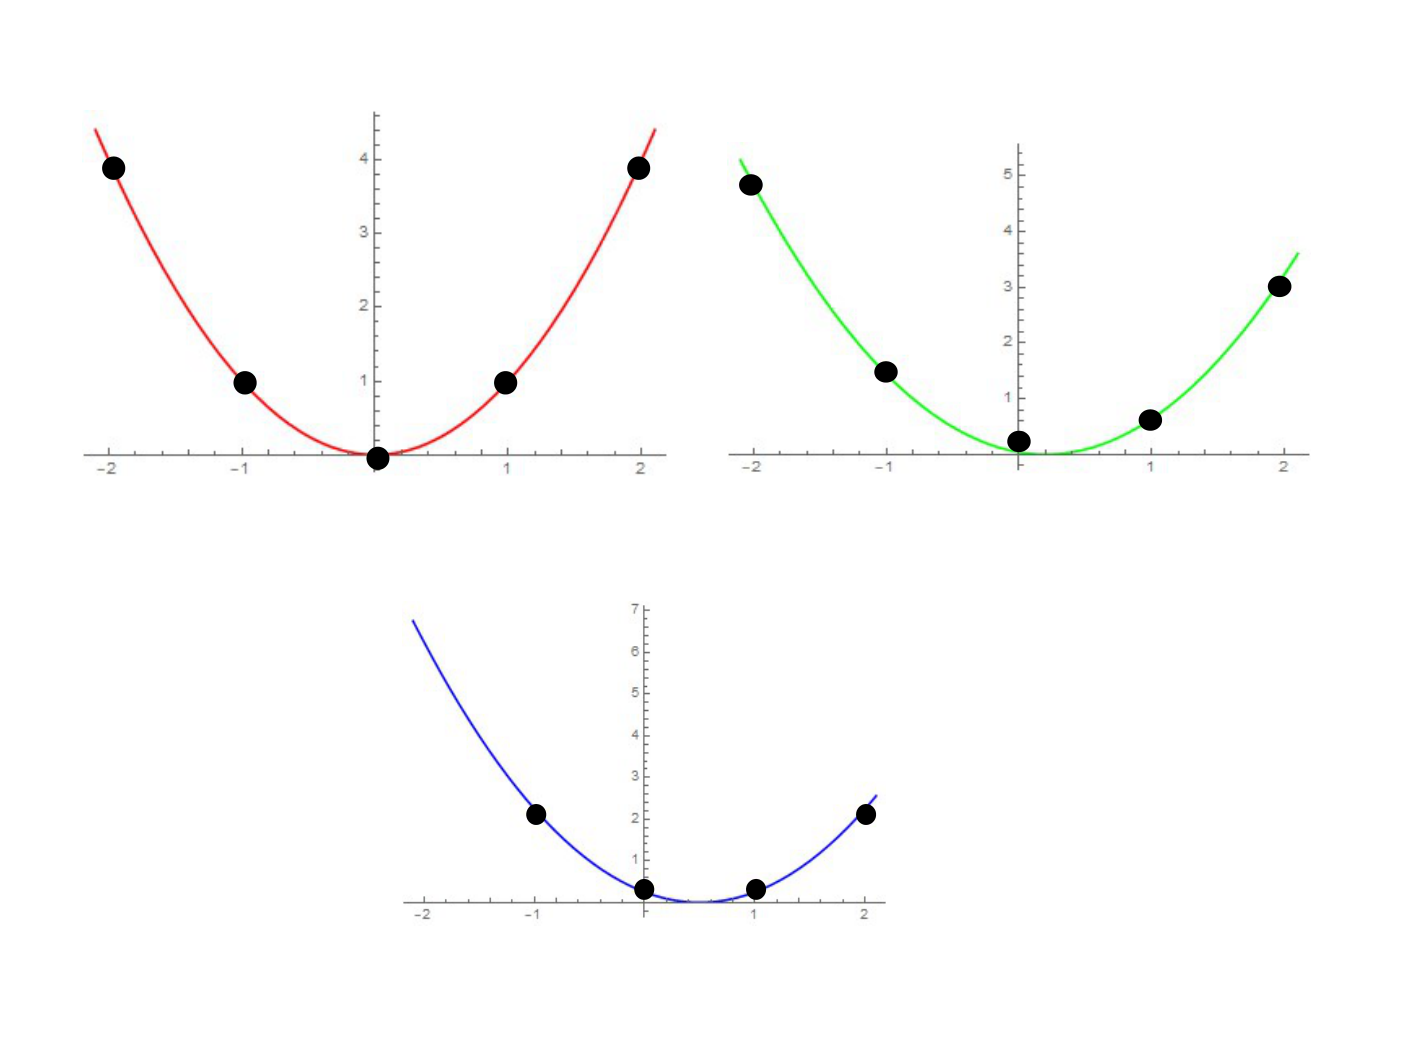
\includegraphics[width=0.85\textwidth]{figures/fig01.png}
  \caption{圆环上粒子的谱作为 $\mathcal{B}=eB/2\pi$ 的函数。左上图给出 $\mathcal{B}=0$ 时的低能谱，它在 $m\to-m$ 下对称。右上图给出 $\mathcal{B}=0.2$ 时的谱，谱中没有对称性。下图给出 $\mathcal{B}=1/2$ 时的谱，此时又有对称性，但对称操作是 $m\to2\mathcal{B}-m=1-m$。一般地，除非 $2\mathcal{B}\in\mathbb{Z}$，否则不会有任何对称性；若 $2\mathcal{B}\in\mathbb{Z}$，则谱在 $m\to2\mathcal{B}-m$ 下对称。（原文 Fig.~1，第 10 页）}
  \label{fig:1}
\end{figure}

第二项是「拓扑项」（topological term）或「$\theta$ 项」（$\theta$-term）的一个例子。经典地，第二项不影响物理预言，因为它是全导数。然而在量子力学层面，它会对物理预言产生重要影响。

我们将分析这个系统的对称性，并比较它们在经典理论与量子理论中的实现方式。

我们先分析经典对称性。由于 $\theta$ 项不影响经典动力学，经典系统具有 $O(2)$ 对称性。我们可以旋转：$R(\alpha):e^{\mathrm{i}\phi}\to e^{\mathrm{i}\alpha}e^{\mathrm{i}\phi}$；或者，如果你愿意，平移 $\phi\to\phi+\alpha$（始终记住 $\alpha$ 与 $\phi$ 只在模去 $2\pi$ 的整数倍的意义下有定义）。如果我们把圆环想成 $x-y$ 平面内以原点为心、螺线管沿 $z$ 轴的圆，那么我们也可以照例取

\begin{equation}
  R(\alpha)=
  \begin{pmatrix}
    \cos\alpha & \sin\alpha\\
    -\sin\alpha & \cos\alpha
  \end{pmatrix}
  \tag{2.4}
  \label{eq:2.4}
\end{equation}

此外我们还可以作「宇称」（parity）或「电荷共轭」（charge conjugation）变换 $P:\phi\to-\phi$。Lagrangian 中的第二项并不是不变的，但这「不要紧」，因为它是全导数。换个说法：$\phi\to-\phi$ 是运动方程的一个对称性。

注意 $O(2)$ 中这些群元素满足

\begin{gather}
  R(\alpha)R(\beta)=R(\alpha+\beta) \notag\\
  P^{2}=1 \notag\\
  PR(\alpha)P=R(-\alpha)
  \tag{2.5}
  \label{eq:2.5}
\end{gather}

而确实，正如我们已经看到的，$O(2)$ 是一个半直积（semidirect product）：

\begin{equation}
  O(2)=SO(2)\rtimes\mathbb{Z}_2
  \tag{2.6}
  \label{eq:2.6}
\end{equation}

其中同态 $\omega:\langle P\rangle\cong\mathbb{Z}_2\to Aut(SO(2))\cong\mathbb{Z}_2$ 把 $\mathbb{Z}_2$ 的非平凡元送到那个把 $R(\alpha)\mapsto R(-\alpha)$ 的外自同构。

\underline{把系统看作场论。}

我们引入这个系统时，把它描述为单个粒子的量子力学。然而重要的是注意到，它也可以被看作量子场论的一个特例。一般地，在场论中我们有一个时空 $M$，而场是 $M$ 上取值于某个目标空间（target space）$\mathcal{X}$ 的函数。（所以「目标空间」这个词的意思不多不少，就是场的余域。）在我们的情形里 $M=\mathbb{R}$，解释为时间实轴，而 $\mathcal{X}$ 是圆。于是我们的场是映射

\begin{equation}
  e^{\mathrm{i}\phi}:M\to S^{1}
  \tag{2.7}
  \label{eq:2.7}
\end{equation}

其中 $M$ 是时间实轴，或者也许是某个时间区间。后面我们还会取 $M$ 为圆。场空间是 $Map[M\to\mathcal{X}]$。由于 $M$ 是时间的一维流形，我们称此为「0+1 维场论」。我们一直把 $\phi\to-\phi$ 称作「宇称」，因为在平面内被约束在圆上的粒子之量子力学语境中，这是恰当的说法。然而，若采取「我们在讨论一个 0+1 维『场论』」的观点，那么最好把这个操作称为「电荷共轭」，因为它对 $U(1)$ 值的场 $e^{\mathrm{i}\phi}$ 取复共轭。

此外还有（在场论解释下）时间平移不变性与时间反演这两种「世界面（worldvolume）对称性」。它们构成群 $\mathbb{R}\rtimes\mathbb{Z}_2$。我们将把它们放到一边。（注意时间反演不是 Lagrangian 中第二项的对称性，但它是运动方程解空间的对称性。）

\underline{量子理论中的对称性。}

现在让我们考虑把「$\theta$ 项」加到 Lagrangian 之后的量子力学。我们的目标是看清该项如何影响量子理论。

我们先在哈密顿量（Hamiltonian）途径中分析量子力学。关于路径积分途径的一些评论见下面的注记。共轭动量（conjugate momentum）是

\begin{equation}
  L=I\dot\phi+\frac{eB}{2\pi}
  \tag{2.8}
  \label{eq:2.8}
\end{equation}

我们用 $L$ 记它，因为可以把它看成角动量。

注意，与平坦规范场的耦合改变了角动量与速度之间的通常关系。现在由 Legendre 变换得到哈密顿量：

\begin{equation}
  \int L\dot\phi\,dt-S=\int\frac{1}{2I}\Big(L-\frac{eB}{2\pi}\Big)^{2}dt
  \tag{2.9}
  \label{eq:2.9}
\end{equation}

量子化之后\footnote{这里可以再加一个常数。它会在量子化故事中引入第二个参数，但与 $\mathcal{B}$ 冗余。} $L\to-\mathrm{i}\hbar\frac{\partial}{\partial\phi}$，于是哈密顿量为

\begin{equation}
  H_{\mathcal{B}}:=\frac{\hbar^{2}}{2I}\Big(-\mathrm{i}\frac{\partial}{\partial\phi}-\mathcal{B}\Big)^{2}
  \tag{2.10}
  \label{eq:2.10}
\end{equation}

其中 $\mathcal{B}:=\frac{eB}{2\pi\hbar}$。

哈密顿量 $H_{\mathcal{B}}$ 的本征函数就是

\begin{equation}
  \Psi_m(\phi)=\frac{1}{\sqrt{2\pi}}e^{\mathrm{i}m\phi}
  \qquad m\in\mathbb{Z}
  \tag{2.11}
  \label{eq:2.11}
\end{equation}

它们给出能量本征态，其能量为

\begin{equation}
  E_m=\frac{\hbar^{2}}{2I}(m-\mathcal{B})^{2}
  \tag{2.12}
  \label{eq:2.12}
\end{equation}

对每个 $m\in\mathbb{Z}$ 恰有一个能量本征态。

% [Tutor Note: (2.9)$\to$(2.10) 这一步省略了代数：由 $L=I\dot\phi+\frac{eB}{2\pi}$ 得 $\dot\phi=(L-\frac{eB}{2\pi})/I$，代回 $H=L\dot\phi-\mathcal{L}$ 才得 $\frac{1}{2I}(L-\frac{eB}{2\pi})^2$；再令 $L\to-\mathrm{i}\hbar\partial_\phi$ 并把 $\frac{eB}{2\pi}$ 除以 $\hbar$ 写成 $\mathcal{B}$，才有 (2.10)。易错之处：$\mathcal{B}$ 里含 $\hbar$，而 $B$ 不含，混用会使 (2.12) 的周期判据从 $2\mathcal{B}\in\mathbb{Z}$ 错成 $2\pi\mathcal{B}\in\mathbb{Z}$；(2.11) 中 $m$ 取整数则来自 $\phi\sim\phi+2\pi$，即目标空间是圆——这正好回答了注 1 末尾的提问。]

\textbf{Remarks（注记）：}

\begin{enumerate}
  \item 作用量 (2.31) 无论对取值于实轴的 $\phi$，还是对取值于圆、满足 $\phi\sim\phi+2\pi$ 的 $\phi$，都完全说得通。作这个选择对于确定我们在描述哪个理论很重要。在上面的分析中——我们究竟在哪里作出了「目标空间是圆」这一选择？\footnote{\emph{答}：如果我们取 $\phi$ 取值于 $\mathbb{R}$ 而非圆的情形，那么对 $m$ 就没有量子化，哈密顿量的谱将是连续的。在这种情形下，Chern-Simons 项在量子力学版本中同样不会影响物理。}
  \item 取 $\phi\sim\phi+2\pi$ 之后，尽管 $\theta$ 项是全导数，它对量子物理仍有非平凡的影响——这一点我们可以从 $B$ 以物理上可观测的方式移动了量子哈密顿量的谱看出来：\emph{这就是我们看出拓扑项要紧的方式。}
  \item 注意当 $2\mathcal{B}$ 为偶数时，能量本征空间是二重简并的，只有位于 $m=\mathcal{B}$ 的基态例外。另一方面，当 $2\mathcal{B}$ 为奇数时，所有能量本征空间都是二重简并的，包括基态。若 $2\mathcal{B}$ 不是整数，则所有能量本征空间都是一维的。见图~\ref{fig:1}。
  \item 整个谱关于 $\mathcal{B}$ 是\emph{周期的}，且平移 $\mathcal{B}\to\mathcal{B}+1$ 等价于 $m\to m+1$。更精确地说，我们可以用在完备基上的作用来定义 Hilbert 空间上的一个酉算符：
\end{enumerate}

\begin{equation}
  U\Psi_m=\Psi_{m+1}
  \tag{2.13}
  \label{eq:2.13}
\end{equation}

以及

\begin{equation}
  UH_{\mathcal{B}}U^{-1}=H_{\mathcal{B}+1}
  \tag{2.14}
  \label{eq:2.14}
\end{equation}

\begin{enumerate}[start=5]
  \item 量子力学问题 (2.31) 与谱 \eqref{eq:2.12} 出现在量子点物理中「Coulomb 阻塞」（Coulomb blockade）的讨论里。参见 Yoshimasa Murayama，\emph{Mesoscopic Systems}，第 10.10 节。
  \item \emph{与高维场论及弦论的关系。} 我们加进来的 $\theta$ 项，在 $1+1$ 维场论中有一个非常有趣的对应物，在那里它被称为与 $B$-场的耦合。它也可以由 $1+1$ 维 Maxwell 理论的 Kaluza-Klein 约化得到：
\end{enumerate}

\begin{equation}
  S=\frac{1}{e^{2}}\int F\ast F+\int\frac{\theta}{2\pi}F
  \tag{2.15}
  \label{eq:2.15}
\end{equation}

在 $1+1$ 维理论中，我们可以取 $A_0=0$ 规范并规范掉对 $x^{1}$ 的依赖，于是在 $S^{1}\times\mathbb{R}$ 上唯一规范不变的量是

\begin{equation}
  e^{\mathrm{i}\phi(t)}=e^{\mathrm{i}\oint_{S^{1}}A}=e^{\mathrm{i}\oint_{S^{1}}A_1dx^{1}}
  \tag{2.16}
  \label{eq:2.16}
\end{equation}

有了这一点，我们可以说

\begin{equation}
  \theta=2\pi\mathcal{B}
  \tag{2.17}
  \label{eq:2.17}
\end{equation}

\textbf{Remark：}更一般地，在 $S^{1}\times\mathbb{R}$ 上的 $1+1$ 维 Yang-Mills 理论中，我们总可以走到 $A_0=0$ 规范，此时唯一规范不变的可观测量是绕圆的和乐（holonomy）的共轭类。

% [Tutor Note: 原文 p.12 注 1 与 p.13 注 5 两处把作用量编号写作 (2.31)，而本片段的作用量是 (2.1)（原书 (2.31) 是后文另一式）。据上下文判断这是作者的交叉引用笔误，译文照原样保留 (2.31) 不擅改，读者应回看 (2.1)。]

$\theta$ 项在 $3+1$ 维规范理论中也有一个密切的对应物。在 $3+1$ 维 Maxwell 理论的情形，我们可以写下

\begin{equation}
  S=\int d^{4}x\,\frac{1}{4e^{2}}F_{\mu\nu}F^{\mu\nu}+\int\frac{\theta}{(2\pi)^{2}}F\wedge F
  \tag{2.18}
  \label{eq:2.18}
\end{equation}

事实上，在存在绝缘体时电磁学的有效理论中，会出现一个非常相似、带 $\theta$ 项的作用量。如果存在宇称和/或时间反演对称性，那么 $\theta$ 为零或 $\pi$，对应于我们的情形 $2\mathcal{B}\in\mathbb{Z}$。于是普通绝缘体与拓扑绝缘体（topological insulator）之间的差别，字面上就是 $2\mathcal{B}$ 为偶数（普通）与为奇数（拓扑）的差别。最后，在描述弱、强相互作用标准模型的 $3+1$ 维 Yang-Mills 理论中，人们可以加入一个类似的 $\theta$ 项。关于自然的一个伟大未解之谜是：标准模型中强相互作用的（有效）theta 角为何小到无法测量。

现在，如果我们考察 $O(2)$ 对称性在量子理论中如何实现，我们会发现一个意外：

% 该编号列表在原 p.13 页末被切断：第 2 项起接续于下一片段（c02）。
\begin{enumerate}
  \item 经典理论具有 $O(2)$ 对称性。
\end{enumerate}
